%%%%%%%%%%%%%%%%%%%%%%%%%%%%%%%%%%%%%%%%%
% This is a template for LaTeX thesis (M.Sc. or PhD) at ZHAW.
% 
% ZHAW thesis template downloaded from:
% https://github.com/matteodelucchi/ZHAW_thesis-template
% 
% University specific changes were made by:
% Matteo Delucchi
%
% Based on a template downloaded from:
% http://www.LaTeXTemplates.com
% 
% Version 2.x major modifications by:
% Vel (vel@latextemplates.com)
%
% This template is based on a template by:
% Steve Gunn (http://users.ecs.soton.ac.uk/srg/softwaretools/document/templates/)
% Sunil Patel (http://www.sunilpatel.co.uk/thesis-template/)
%
% Template license:
% CC BY-NC-SA 3.0 (http://creativecommons.org/licenses/by-nc-sa/3.0/)
%
%%%%%%%%%%%%%%%%%%%%%%%%%%%%%%%%%%%%%%%%%

%----------------------------------------------------------------------------------------
%	PACKAGES AND OTHER DOCUMENT CONFIGURATIONS
%----------------------------------------------------------------------------------------

\documentclass[
11pt, % The default document font size, options: 10pt, 11pt, 12pt
oneside, % Two side (alternating margins) for binding by default, uncomment to switch to one side
english, % ngerman for German
singlespacing, % Single line spacing, alternatives: onehalfspacing or doublespacing
%draft, % Uncomment to enable draft mode (no pictures, no links, overfull hboxes indicated)
%nolistspacing, % If the document is onehalfspacing or doublespacing, uncomment this to set spacing in lists to single
%liststotoc, % Uncomment to add the list of figures/tables/etc to the table of contents
%toctotoc, % Uncomment to add the main table of contents to the table of contents
%parskip, % Uncomment to add space between paragraphs
%nohyperref, % Uncomment to not load the hyperref package
headsepline, % Uncomment to get a line under the header
%chapterinoneline, % Uncomment to place the chapter title next to the number on one line
%consistentlayout, % Uncomment to change the layout of the declaration, abstract and acknowledgements pages to match the default layout
]{Classfile} % The class file specifying the document structure

\usepackage{titlesec}

\titleformat{\chapter}[display]
  {\Huge\bfseries}
  {}
  {0pt}
  {\thechapter.\ }

\titleformat{name=\chapter,numberless}[display]
  {\Huge\bfseries}
  {}
  {0pt}
  {}

\usepackage[utf8]{inputenc} % Required for inputting international characters
\usepackage[T1]{fontenc} % Output font encoding for international characters
\usepackage{xcolor}


%\usepackage[x-5pg]{pdfx} %for PDF-X support. Has problems with xcolor and hyperref
%\usepackage{subfigure}
\usepackage{caption}
\usepackage{subcaption}

\usepackage{mathpazo} % Use the Palatino font by default

\usepackage[backend=biber,  % Use the bibtex backend with the authoryear citation style (which resembles APA)
sorting=nyt, % numbers the reference in order of their appearance in the document. Troubleshoot with deleting all *.aux and *.bbl files and rebuild.
style=ieee,
natbib=true]{biblatex}

\addbibresource{Bibliography.bib} % The filename of the bibliography

\usepackage[autostyle=true]{csquotes} % Required to generate language-dependent quotes in the bibliography

\usepackage{pdfpages}

\usepackage{todonotes}
\setlength{\marginparwidth}{2.5cm} % uncomment this if the todonotes are out of margins (cut off page)

\usepackage{listings}


\definecolor{codegreen}{rgb}{0,0.6,0}
\definecolor{codegray}{rgb}{0.5,0.5,0.5}
\definecolor{codepurple}{rgb}{0.58,0,0.82}
\definecolor{backcolour}{rgb}{0.921, 0.929, 0.937} %0.95,0.95,0.92

\lstdefinestyle{mystyle}{
backgroundcolor=\color{backcolour},   
commentstyle=\color{codegreen},
keywordstyle=\color{magenta},
numberstyle=\tiny\color{codegray},
stringstyle=\color{codepurple},
basicstyle=\ttfamily\footnotesize,
breakatwhitespace=false,         
breaklines=true,                 
captionpos=b,                    
keepspaces=true,                 
numbers=left,                    
numbersep=5pt,                  
showspaces=false,                
showstringspaces=false,
showtabs=false,                  
tabsize=2
}

\lstset{style=mystyle}

\usepackage{makecell} % formatting tables





%----------------------------------------------------------------------------------------
%	MARGIN SETTINGS
%----------------------------------------------------------------------------------------

\geometry{
paper=a4paper, % Change to letterpaper for US letter
inner=2.5cm, % Inner margin
outer=3.8cm, % Outer margin
bindingoffset=.5cm, % Binding offset
top=1.5cm, % Top margin
bottom=1.5cm, % Bottom margin
%showframe, % Uncomment to show how the type block is set on the page
}


%----------------------------------------------------------------------------------------
%	THESIS INFORMATION
%----------------------------------------------------------------------------------------

\thesistitle{Automatic generation of web applications from Excel documents with Microsoft Graph} % Your thesis title, this is used in the title and abstract, print it elsewhere with \ttitle
\supervisor{\textsc{Dr. Prof Hans Peter-Hutter}} % Your supervisor's name, this is used in the title page, print it elsewhere with \supname
\examiner{\textsc{Dr. Michael Wahler}} % Your examiner's name, this is not currently used anywhere in the template, print it elsewhere with \examname
\degree{MSE Computer Science} % Your degree name (Doctor of Philosophy or Master of Science), this is used in the title page and abstract, print it elsewhere with \degreename
\author{\textsc{Martin Frick}} % Your name, this is used in the title page and abstract, print it elsewhere with \authorname
\addresses{} % Your address, this is not currently used anywhere in the template, print it elsewhere with \addressname

\subject{} % Your subject area, this is not currently used anywhere in the template, print it elsewhere with \subjectname
\keywords{} % Keywords for your thesis, this is not currently used anywhere in the template, print it elsewhere with \keywordnames
\university{Zurich University of Applied Sciences} % Your university's name and URL, this is used in the title page and abstract, print it elsewhere with \univname
\universitygerman{Z{\"u}rcher Hochschule f{\"u}r Angewandte Wissenschaften}% Your university's name in german and URL, this is used in the german abstract (Zusammenfassung), print it elsewhere with \univnameger
\department{} % Your department's name and URL, this is used in the title page and abstract, print it elsewhere with \deptname
\group{} % Your research group's name and URL, this is used in the title page, print it elsewhere with \groupname
\faculty{Institute of Information Technology (InIT)
} % Your faculty's name and URL, this is used in the title page and abstract, print it elsewhere with \facname

\AtBeginDocument{
\hypersetup{pdftitle=\ttitle} % Set the PDF's title to your title
\hypersetup{pdfauthor=\authorname} % Set the PDF's author to your name
\hypersetup{pdfkeywords=\keywordnames} % Set the PDF's keywords to your keywords
}

\begin{document}

\frontmatter % Use roman page numbering style (i, ii, iii, iv...) for the pre-content pages

\pagestyle{plain} % Default to the plain heading style until the thesis style is called for the body content

%----------------------------------------------------------------------------------------
%	TITLE PAGE
%----------------------------------------------------------------------------------------

\begin{titlepage}
\begin{center}

\begin{figure}
\centering

\includegraphics[width=0.15\textwidth]{Figures/ZHAW_Logo.png} % Universtiy Logo, Adapted from: https://upload.wikimedia.org/wikipedia/commons/thumb/e/e6/ZHAW_Logo.svg/879px-ZHAW_Logo.svg.png
\end{figure}

\vspace*{.06\textheight}
{\scshape\LARGE \univname\par}\vspace{1.5cm} % University name
\textsc{\Large VT2}\\[0.5cm] % Thesis type

\HRule \\[0.4cm] % Horizontal line
{\huge \bfseries \ttitle\par}\vspace{0.4cm} % Thesis title
\HRule \\[1.5cm] % Horizontal line
 

\emph{Submitted by:}\\
{\authorname} % Author name - remove the \href bracket to remove the link
\\{15-725-161} \\[1.5cm]


\emph{Advisor:} \\
{\examname} % Supervisor name - remove the \href bracket to remove the link  

 
 \emph{Supervisor:} \\
{\supname}\\[1.5cm] % Supervisor name - remove the \href bracket to remove the link  


\facname\\
\degreename\\[2cm]% Research group name and department name

 
\vfill

{\large \today}\\ % Date
%\includegraphics{Logo} % University/department logo - uncomment to place it
 
\vfill
\end{center}
\end{titlepage}


%----------------------------------------------------------------------------------------
%	ABSTRACT PAGE
%----------------------------------------------------------------------------------------

\begin{abstract}
\addchaptertocentry{\abstractname} % Add the abstract to the table of contents
tbd
\end{abstract}


%----------------------------------------------------------------------------------------
%	LIST OF CONTENTS/FIGURES/TABLES PAGES
%----------------------------------------------------------------------------------------

\tableofcontents % Prints the main table of contents

\listoffigures % Prints the list of figures

\listoftables % Prints the list of tables

%----------------------------------------------------------------------------------------
%	ABBREVIATIONS
%----------------------------------------------------------------------------------------

\begin{abbreviations}{ll} % Include a list of abbreviations (a table of two columns)

\textbf{LAH} & \textbf{L}ist \textbf{A}bbreviations \textbf{H}ere\\
\textbf{WSF} & \textbf{W}hat (it) \textbf{S}tands \textbf{F}or\\


\end{abbreviations}


%----------------------------------------------------------------------------------------
%	THESIS CONTENT - CHAPTERS
%----------------------------------------------------------------------------------------

\mainmatter % Begin numeric (1,2,3...) page numbering

\pagestyle{thesis} % Return the page headers back to the "thesis" style

% Include the chapters of the thesis as separate files from the Chapters folder
% Uncomment the lines as you write the chapters

% Chapter 1

\chapter{Introduction} % Main chapter title

\label{Introduction} % For referencing the chapter elsewhere, use \ref{Chapter1} 

%----------------------------------------------------------------------------------------

% Define some commands to keep the formatting separated from the content 
\newcommand{\keyword}[1]{\textbf{#1}}
\newcommand{\tabhead}[1]{\textbf{#1}}
\newcommand{\code}[1]{\texttt{#1}}
\newcommand{\file}[1]{\texttt{\bfseries#1}}
\newcommand{\option}[1]{\texttt{\itshape#1}}

%----------------------------------------------------------------------------------------

\section{Motivation}
Digitalisation places a special emphasis on companies' ability to react to changes in circumstances, such as changes in the law or changing customer needs. In the near future, business models that are currently successful may not necessarily work in rapidly changing environments \cite{BBA}.

Typically, companies which are not digitally native rely on third-party software. To adapt their products or services to the changing demands, they have a tedious process. If they are too slow, these companies may miss out on key business opportunities, while if they are too fast, they may fail to deliver quality software \cite{BBA}.

Model-driven engineering (MDE) can come here in place in order to reduce time from requirements to implementation. MDE is defined as a process in which domain experts such as product managers capture requirements through models. In theory, these models can be automatically transformed in executable code. However, the reality is that MDE is rarely used in general software development today, but rather in some niches. It is assumed that the success of MDE in these niches depends on the use of domain-specific languages that allow domain experts to express requirements in a formal language that is natural to both them and software developers, as in contrast to other domains that lack a modelling language as common basis \cite{BBA}.

Microsoft Office documents could serve as such a common basis, as they have a high acceptance in the working world. Also, Office documents often contain valuable domain data and business logic which is later manually converted into code by software developers. When applying MDE, domain experts could thus easily reflect changes in the environment in a Office document from which an updated version of the software can be automatically be generated.  In this way, companies are enabling themselves to quickly respond to changing business requirements by integrating business artefacts from domain-specific languages (e.g Microsoft Excel.) into their software development life cycle \cite{BBA}.

There are existing approaches how Microsoft Excel could be used as a micro service with the help of a python package called "formulas" \cite{BBA}. With the use of code generation and model interpretation it was made possible to integrate an Excel document into an existing application as first-class modeling artefact.
However, first tests have shown that it is a rather slow solution performancewise. Also, not all functions types are are supported which can be performed by Microsoft Excel. Thus, it is necessary to find other solutions which are able to overcome these limitations \cite{BBA}. 





%----------------------------------------------------------------------------------------

\section{Motivation Example}

The validation of the different approaches is based on an example from industry that uses an Excel document to calculate the required spare parts for electrical devices. The calculations defined in the Excel document are to be made available as a micro-service. 
The spare parts listed in the Excel file generate costs for their storage and preservation. It is therefore a natural goal to have as few of them as possible. On the other hand, the largest possible stock should be ensured so that in case of failures, they can be repaired immediately, thus reducing the economic impact. According to various input data, the Excel document calculates the optimal stock of spare parts so that the total costs are minimised.

...

\section{Objective and Structure}

%hier evtl noch besser an Motivation Teil anknüpfen
The aim of this VT is to create a web application that can interact with an Excel document that is available as a micro service. The user of the web application should be able to call up the micro service by entering the inputs in an input mask. When the service is called, it should write the parameters into predefined fields of the Excel file, calculate the formulas in the file and return predefined cell values as a result and display them in the UI of the web application. 
The interaction with the Excel document is to be based on the "model at runtime" principle. Microsoft Graph is to be used for interaction with the model (i.e. the Excel document). Microsoft Graph provides a REST API for Excel documents stored in the cloud to enable their integration into web applications. The performance and limitations of the technology will be evaluated and compared  to existing solution which make us of the python package "formulas" \cite{BBA}.

Furthermore, it should be possible to generate the UI of the web application automatically from the Excel document (e.g. from predefined input and output fields of the Excel document). Alternatively, an approach should be developed that allows the Excel document to be integrated into an existing web application. In this case, inputs for calculations should not come from an input mask, but should be obtained from an integrated database that has the required data.

%To be able to do research on the topic, Chapter 2 summarises the theoretical foundation for MDSE in general and regarding to the two principles of models at compile time and models at runtime. After the theoretical foundation, chapter 3 gives an insight into the specific case of using Microsoft Office documents in the context of MDSE. In Chapter 5, possible technologies for using Microsoft Office documents are evaluated in terms of compile time models and runtime models. The technologies are evaluated regarding the aspects defined in chapter 4. Finally, in chapter 6, a summary and a hint for future work are given.


\section{Methodology}

tbd

%To answer the research question appropriately, a literature review is conducted to gain an understanding of MDSE and its theoretical foundation. The basic understanding of the topic gained subsequently enables to do research on using Microsoft Office in the context of MDSE. Furthermore, possible technologies to interact with documents are evaluated according to the following aspects:
%•	Dependence on a specific Office version
%•	License costs
%•	Performance
%•	Ease of use
%•	Completeness of generated code
%•	Testability
%For each of the technologies found, a description of how the technology works and helps to implement the desired principle is given. Also, the tools and libraries needed for the performed evaluation are documented. Where possible, the feasibility of the tech-nology for the desired principles is investigated with a short example programme. Final-ly, limitations of the chosen technologies are shown.



% Chapter Template

\chapter{Microsoft Graph foundations} % Main chapter title

\label{Chapter2} % Change X to a consecutive number; for referencing this chapter elsewhere, use \ref{ChapterX}

%----------------------------------------------------------------------------------------
%	SECTION 1
%----------------------------------------------------------------------------------------

\section{Overview}

Microsoft Graph is a gateway to data and intelligence in Microsoft 365. It provides a unified programmability model that you can use to access data in Microsoft 365. Microsoft Graph can further be used to build apps for organizations and consumers that interact with millions of users \cite{MSGraphOverview} .

In Microsoft Graph there is a single endpoint that provides access to data in the Microsoft Cloud, including Microsoft Office. REST APIs can be used to access the endpoint and build applications that enable manipulating an Excel workbook for example. As part of Microsoft Graph, organisations can also manage user and device identity, access, compliance, and security, as well as protect against data leakage and loss \cite{MSGraphOverview}.

Inbound Connectors for Microsoft Graph carry data inside the Microsoft cloud and deliver it to Microsoft Graph services and applications, such as Microsoft Search. Apart from that, many common data sources outside the Microsoft universe are available via connectors, such as Google Drive, Jira and Salesforce \cite{MSGraphOverview}.

For Azure development tools, you can use the cached data as a source of data for developing intelligent applications.
Microsoft Graph API, connectors, and Data Connect together form the basis of the 365 platform. As a result of your ability to access Microsoft Graph data and other datasets, you can get insights and create your own applications \cite{MSGraphOverview}.


With regards to the objective of this VT, Microsoft Graph can be used by the web-based application to read and modify Excel workbooks stored on OneDrive for Business, a SharePoint site, or a group drive. A workbook can be accessed through the Drive API by specifying its location in the URL. The format of the URL looks as follows:
\\

https://graph.microsoft.com/v1.0/me/drive/items/{id}/workbook/  
\\[0.5cm]
Each file in OneDrive gets an id assigned which needs to be considered in the path. By using the standard REST APIs, a user can access a set of Excel objects such as a range of cells and perform CRUD operations (create, read, update, and delete) on the workbook. 


%----------------------------------------------------------------------------------------
%	SECTION 2
%----------------------------------------------------------------------------------------

\section{Authentication and authorization}

Your users and customers can utilize the Microsoft Identity Platform to sign into your applications using their Microsoft identities or social accounts, and give them access to Microsoft Graph. In the process OAuth 2.0 and OpenID Connect (OIDC) flows are used for Authentication and authorization respectively \cite{MSIDP}. In OAuth 2.0 the following roles as shown in \ref{fig:roles for Microsoft Graph} are defined in the context of Microsoft Graph \cite{MSOAuthOIDr}:

\begin{figure}[h!]
  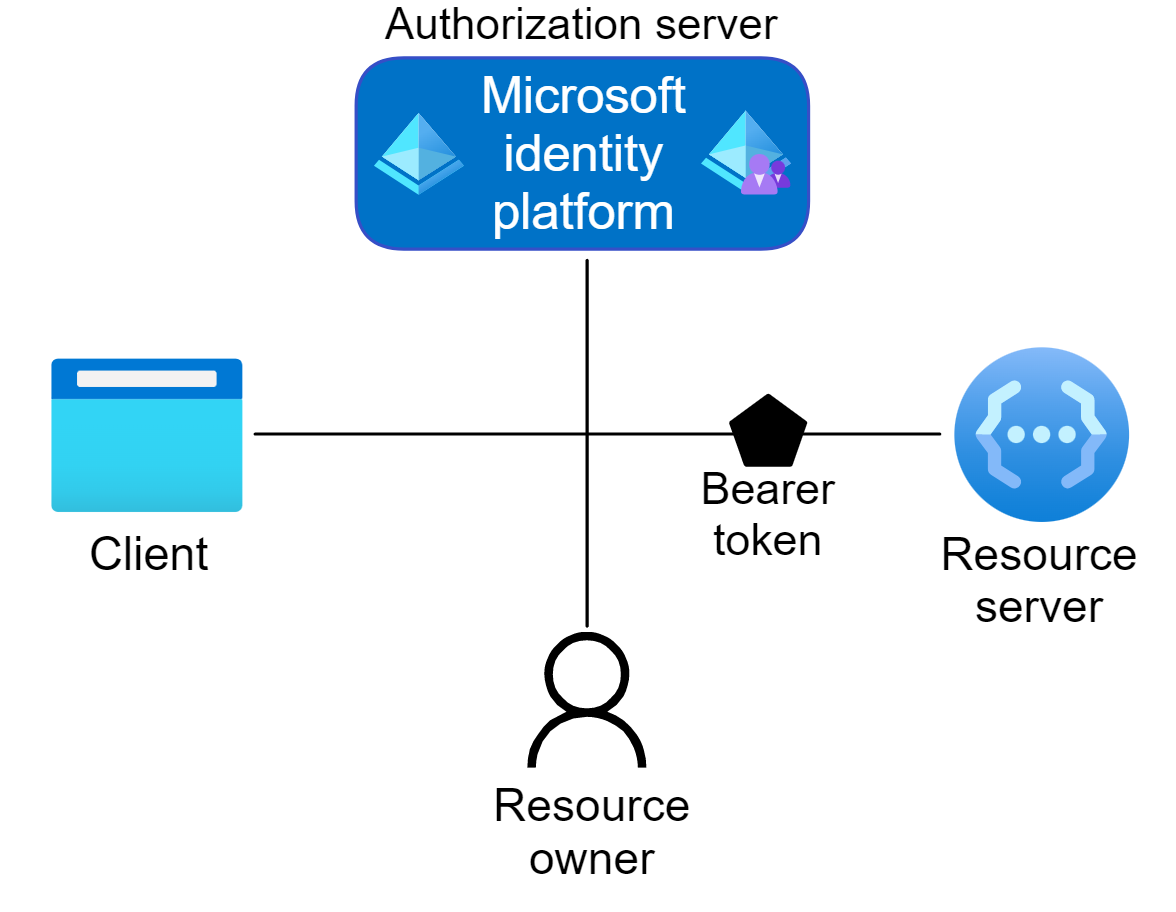
\includegraphics[scale=0.9]{Figures/OAuth roles.png}
  \caption{roles for Microsoft Graph}
  \label{OAuth 2.0 roles for Microsoft Graph}
\end{figure}

\begin{itemize}
 \item Authorisation server: The Microsoft Identity Platform serves as the authorization server. In addition, it performs the function of an identity provider (IdP) since it maintains Microsoft accounts and oversees the trust relationship between parties during the authentication process. Authorization servers create security tokens after a user logs in (authenticates) to grant, deny or revoke access to resources (authorization) \cite{MSOAuthOIDr}.
 \item Client: The client in this context is your application you created and registered on the Microsoft Identity platform. It requests access to protected resources as soon as it being used. Depending on the client, it can be a server-based web application, a user-facing one-page web application, or a web API that interacts with another web API \cite{MSOAuthOIDr}. 
 \item Ressource Owner: An application user is usually the resource owner in an authentication flow. Your application wants to access the users data on the ressource owners behalf. The owner of the resource can grant or deny your application (the client) access to the resources it owns \cite{MSOAuthOIDr}. 
 \item Resource server: The resource server hosts or provides access to data owned by a resource owner. A data store is usually preceded by a web API serving as a resource server. Access to resources is controlled by the resource server using information in owner tokens issued by the authentication server \cite{MSOAuthOIDr}. 
\end{itemize}

A flow of authentication uses bearer tokens to guarantee identification (authentication) and to grant or deny access to protected resources (authorization). JSON Web Tokens (JWT) are formatted for bearer tokens in Microsoft Identity Platform. A bearer token may be one of three types used by the Microsoft Identity Platform as a security token:

\begin{itemize}
 \item Access tokens: The authorisation server issues access tokens to the client application. The client then passes these tokens on to the resource server. Access tokens are further sent from Authorisation servers to the client to declare which resources and APIs your app has access to \cite{MSOAuthOIDr}. It includes information (claims) that is verified using web APIs protected by the platform, such as Microsoft Graph, to determine whether the user has the necessary permissions to execute the request. An HTTP request with an Authorization header must include the access token attached as a Bearer token \cite{MSAA}.
 \item ID tokens: The client application receives ID tokens from the authorisation server. A client uses an ID token to enroll users and to gain basic information about them.
 \item Refresh tokens: Clients use refresh tokens to request new access and ID tokens from the authorization server.
\end{itemize}


Obtaining security tokens from Microsoft Identity Platform is the crucial step in accessing Microsoft Graph. Security tokens for Microsoft Graph can only be acquired if your application is registered with the Microsoft Identity Platform and authorised to access them by either a user or administrator. Through registration, your application (client) can trust the security tokens issued by the Microsoft Identity Platform \cite{MSAA}.

It is mandatory for your application to be registered in the Azure Portal as through registration, you connect your application to Microsoft Identity Platform and define the information it uses for security token retrieval, including:

\begin{itemize}
 \item An application ID that is unique to your application.
 \item Redirect URI/URL: One or more endpoints from which the Microsoft Identity Platform responds to your application.
 \item Client secret: Your application will use your client secret to authenticate to the Microsoft Identity Platform using a password or public/private key pair \cite{MSAA}.
\end{itemize}

When it comes to choosing Microsoft Graph permissions for your application, it is up to you as a developer to select these permissions in the Azure Portal. An administrator, or depending on the scenario a user, is given the option to accept these permissions when they log into your application. Users can grant your application access to the requested resources and APIs if they agree. An administrator can preapprove permissions for applications that access resources without requiring a user to log in before. There are two types of permissions in Microsoft Graph which are delegated and application permissions \cite{MSAA}.

Applications with logged-in users use delegates permissions. Users or administrators must approve the application's permissions in order for Microsoft Graph to work with these applications. The application can then act as the logged-in user. Non-administrative users can approve some delegated permissions, but some higher-privileged permissions require administrative approval \cite{MSAA}.

There can also be applications running without an logged-in user. These applications utilize application permissions. Examples include background services and daemons. Only administrators can approve application permissions \cite{MSAA}.

For managing token interactions with the Microsoft Identity Platform, developers typically use authentication libraries. As a developer, you can focus on the functionality of your application while authentication libraries handle many protocol details such as cookie processing, token caching, and maintaining secure connections. Several Microsoft open source client libraries are also available \cite{MSAA}.

In order to use the Microsoft identity platform endpoint there are Microsoft Authentication Library (MSAL) client libraries for .NET. As part of their implementation of the Microsoft Authentication Library (MSAL), authentication providers implement the code required to acquire a token, handle errors such as incremental consent, expired passwords, and conditional access, and set the HTTP request authorisation header. Listed below are the providers that correspond to the different types of applications. According to the table each scenario and application type match a different authentication provider \cite{MSAuthPr}.

\begin{figure}[h!]
  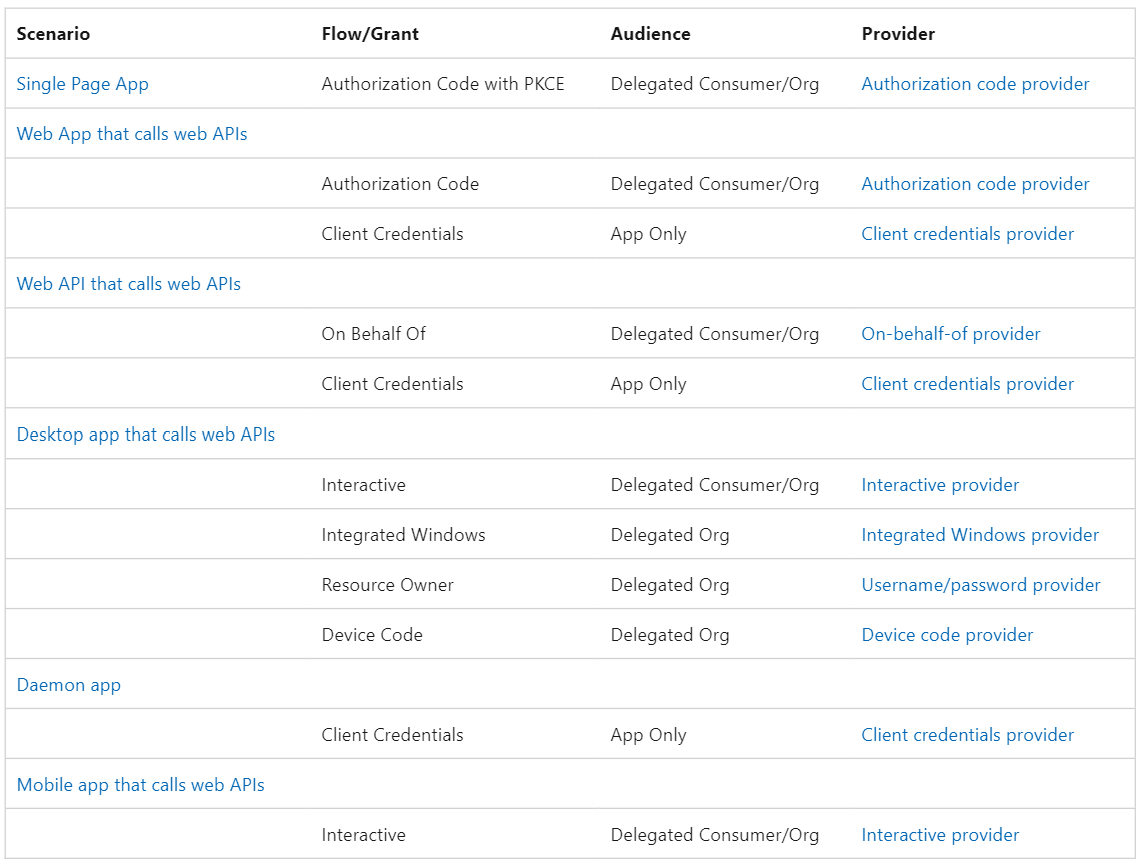
\includegraphics[scale=0.95]{Figures/Authentication providers.png}
  \caption{Authentication providers according to scenario}
  \label{fig:Authentication providers according to scenario}
\end{figure}

Depending on the selected authentication flow and the according provider, the user will be asked to login in his Microsoft account so that the web app can obtain an access token or the application is enabled to run without user interaction. The former is for example the case for the authorization code provider, while the latter is the case for the client credentials provider \cite{MSAuthPr}.









 
\chapter{Proof of concept: Interacting with Excel documents with Microsoft Graph} % Main chapter title

\label{Proof of concept1} % Change X to a consecutive number; for referencing this chapter elsewhere, use \ref{ChapterX}

%----------------------------------------------------------------------------------------
%	SECTION 1
%----------------------------------------------------------------------------------------

\section{App registration and permission granting on the Azure Portal}

Below it can be seen how the app registration process looks like on the Azure Portal. There needs to be an app name defined as well as supported account types. Also there can optionally be an redirect URI defined where the authentication response goes to after a successful authentication \cite{MSAppReg}. 

\begin{figure}[h!]
  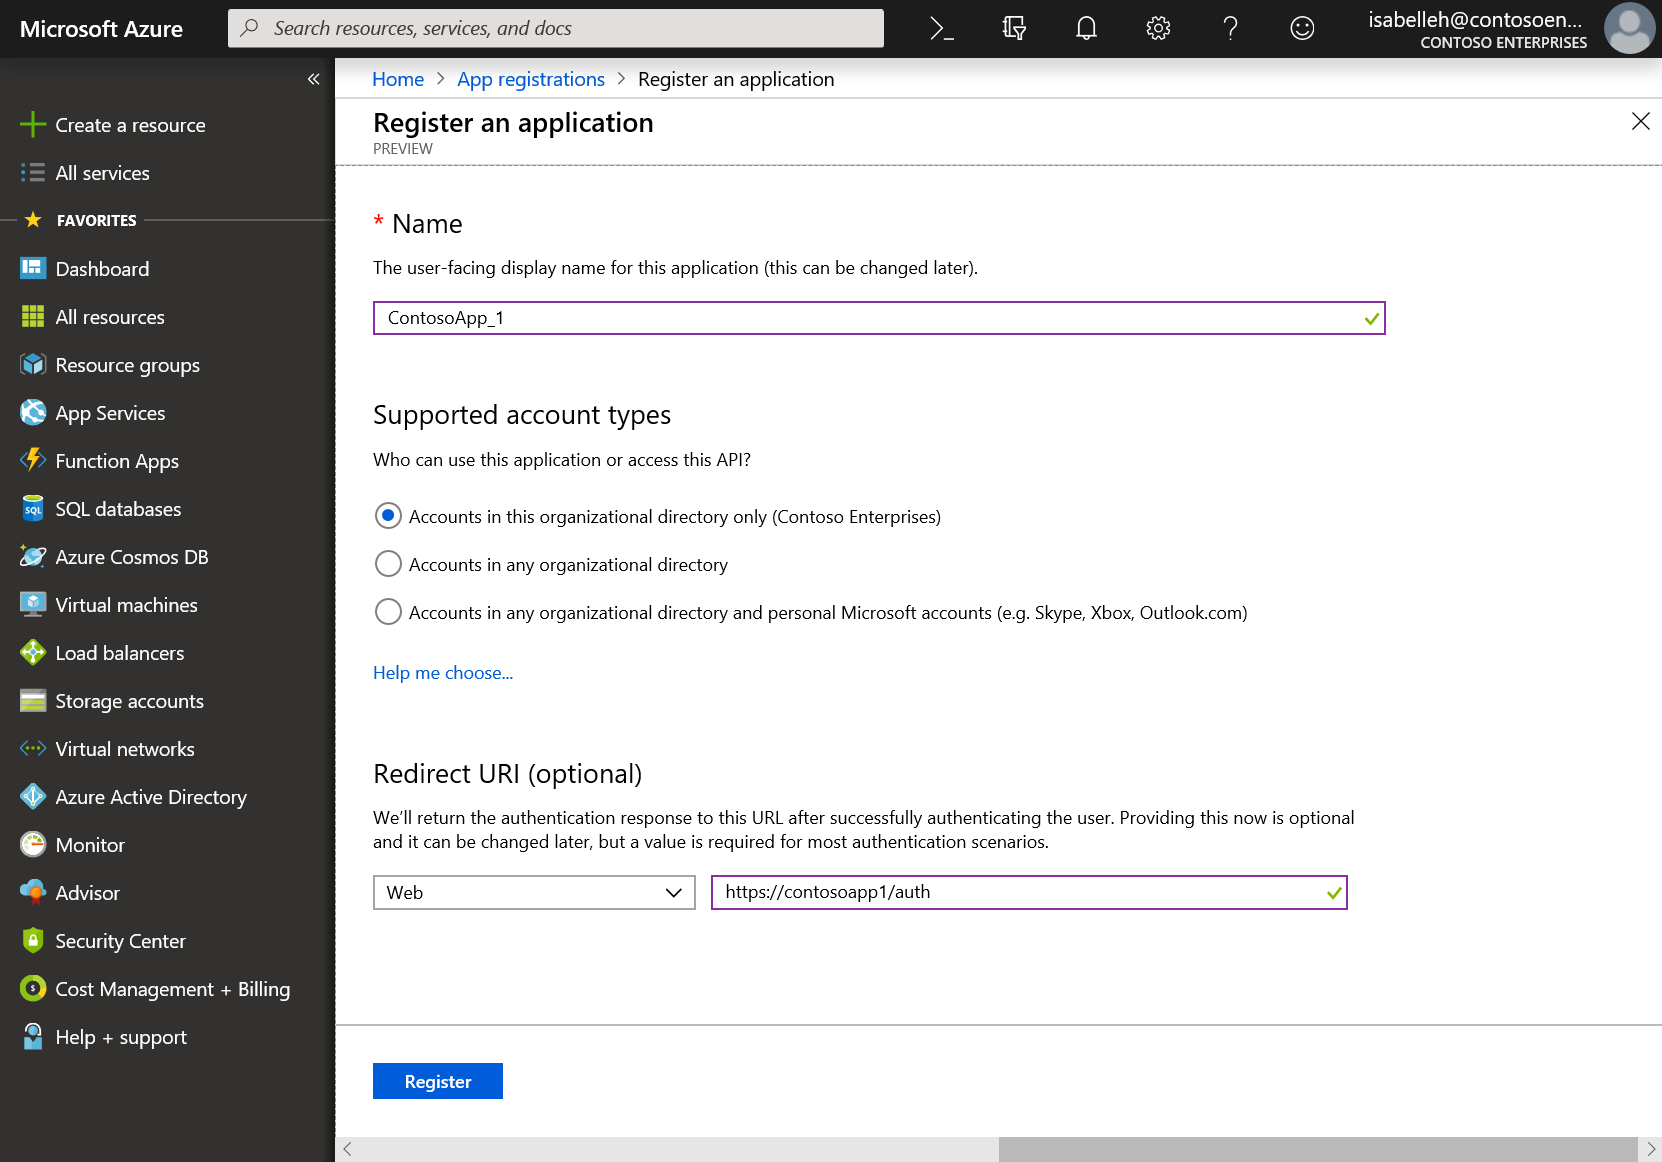
\includegraphics[scale=0.45]{Figures/new-app-registration-expanded.png}
  \caption{App registration process}
  \label{fig:App registration process}
\end{figure}

For the web-app to be created it makes sense to use client credentials authentication provider, as it is favourable to have authentication without user interaction. In that case a Share-point online (SPO) license is required in order to use the Graph. Such a license is only available in work or school accounts. Attempts with a private account and an Office 365 subscription failed, as for private accounts its not possible to have an SPO license. As at ZHAW, the use of Graph is restricted by System admins, such an admin needs to be contacted. The system admin has to create a test user, assign the required SPO license to that test user and register the application. 

The system admin is further required to create a client secret as shown below. The application uses to client secret to authenticate at the Microsoft Identity Platform.

\begin{figure}[h!]
  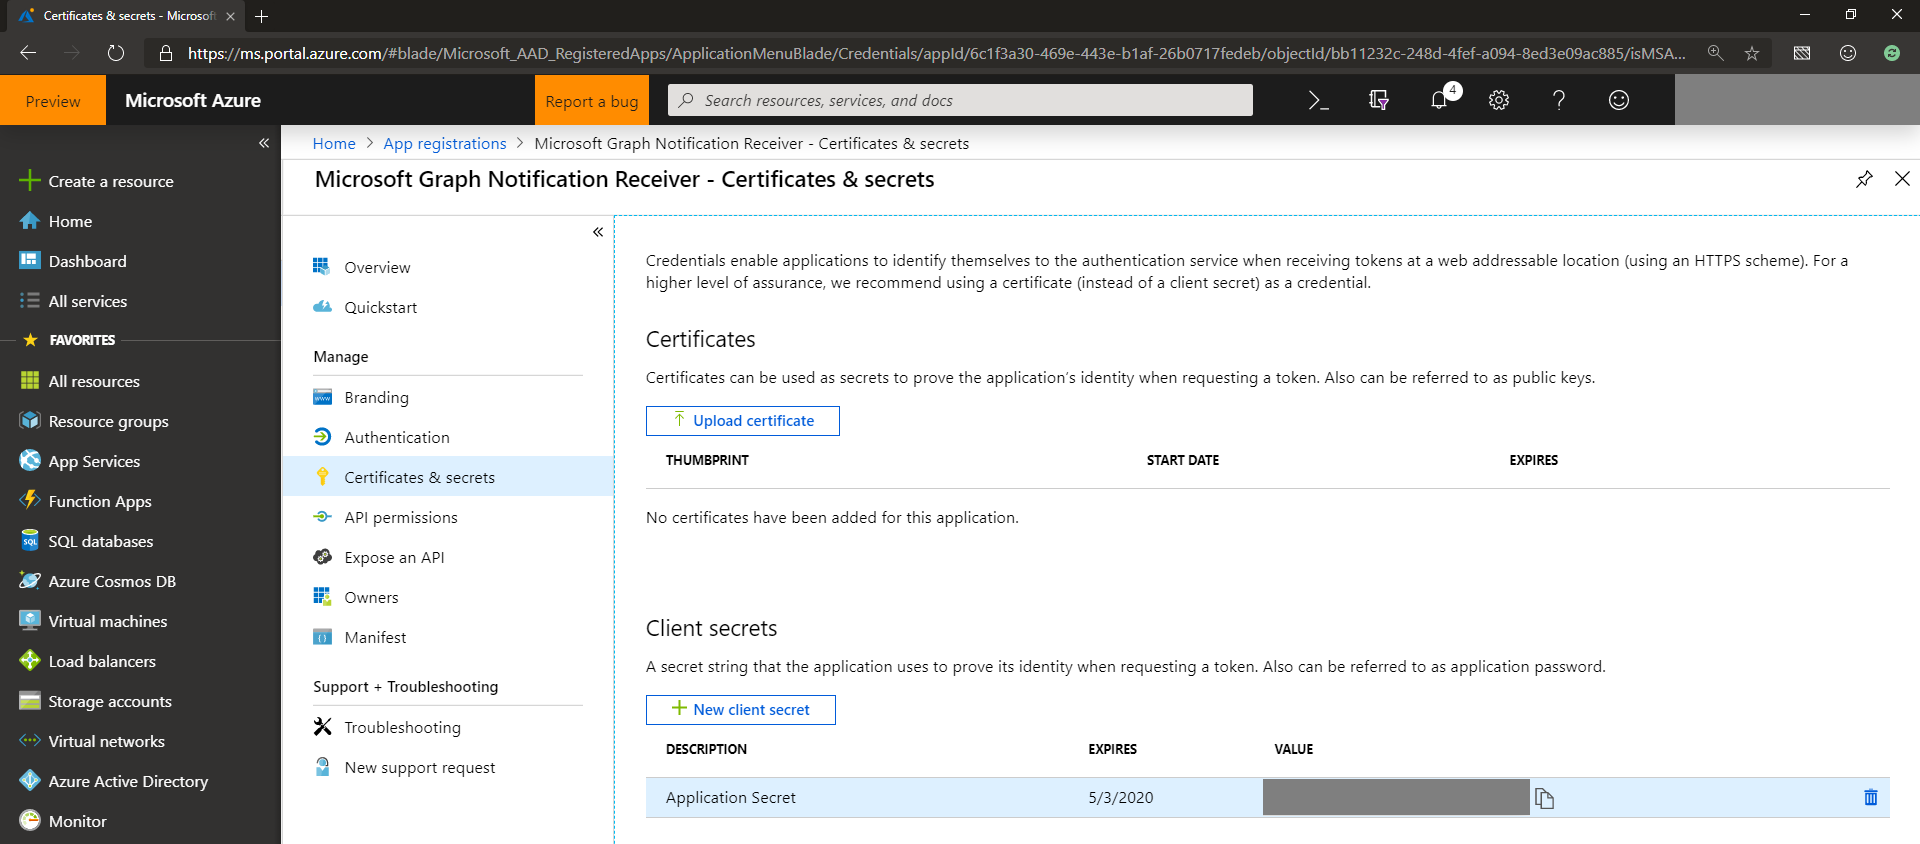
\includegraphics[scale=0.275]{Figures/client-secret.png}
  \caption{Client secret}
  \label{fig:Creation of client secret}
\end{figure}

Also, the API permissions need to be defined in the app, so they can be written to the access token which is needed for every http request. This can be done in the "API permission section" as shown as below:

\begin{figure}[h!]
  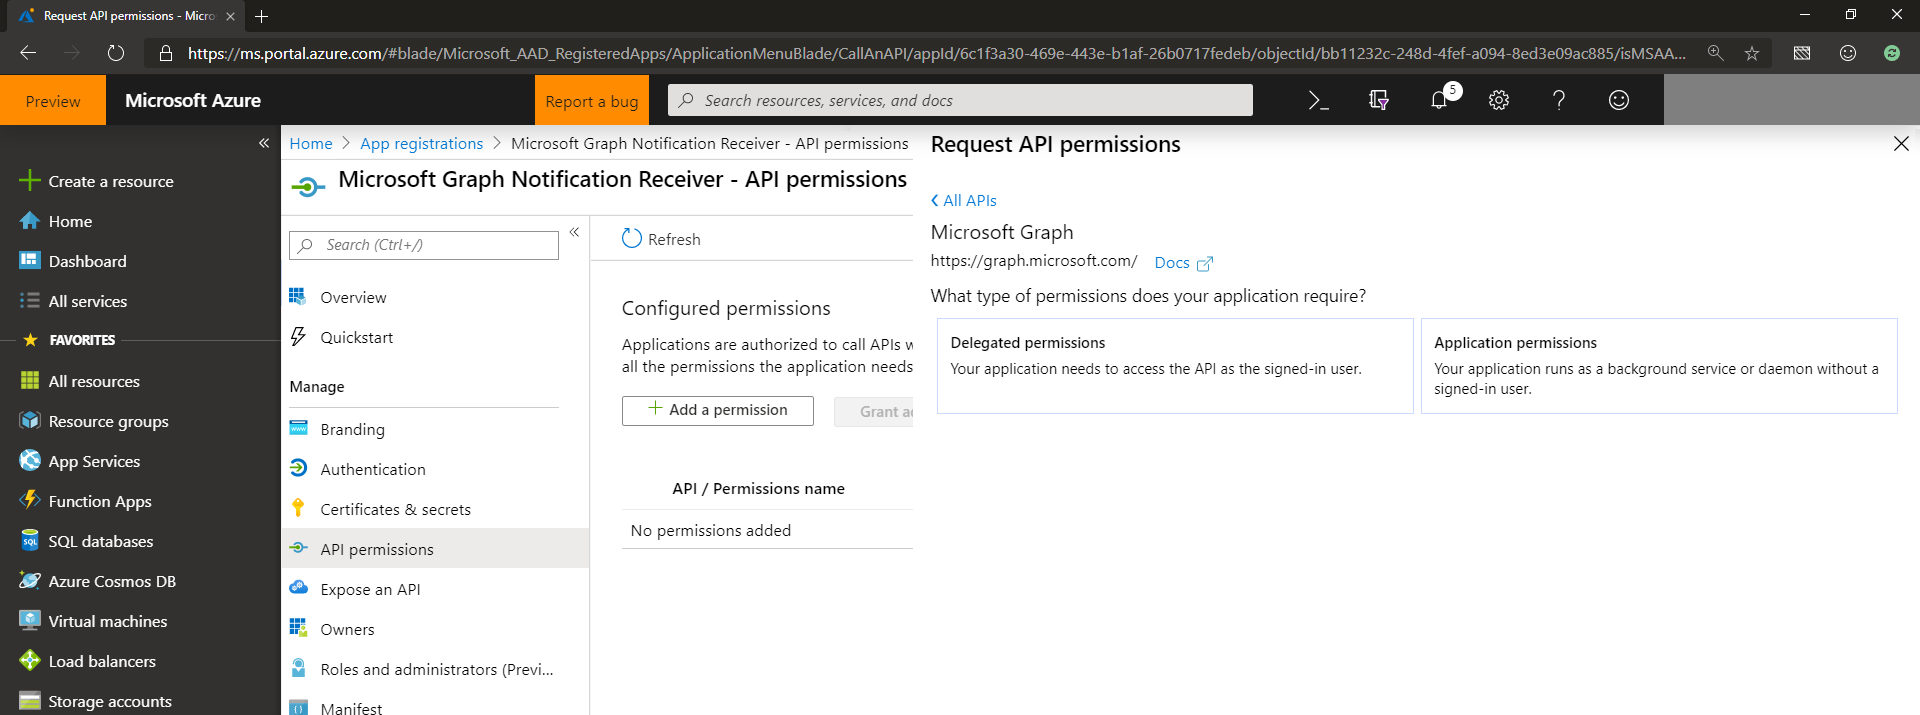
\includegraphics[scale=0.275]{Figures/notifications-api-permissions.png}
  \caption{API permissions}
  \label{fig: Adding API permissions}
\end{figure}

Following API permissions need to be selected in order to access the Excel document. The permission also need to be consented by the system admin:


\begin{longtable}[]{@{}lll@{}}
\toprule
Permission Name & Type & Description\tabularnewline
\midrule
\endhead
Access.Review.ReadWrite.All & Application & Manage all access reviews\tabularnewline
Directory.Read.All & Application & Read directory data\tabularnewline
Files.ReadWrite.All & Application & Read and write files in all site collections\tabularnewline
Sites.Read.All & Application & Read items in all site collections\tabularnewline
User.Read & Delegated & Sign in and read user profile\tabularnewline
User.Read.All & Application & Read all users' full profile\tabularnewline
\bottomrule
\caption{Required API permissions}
\label{Required API permissions}
\end{longtable}

After the application registration has been completed, the program to interact with the Excel document can be implemented. In the code snippet below from the Microsoft documentation it can be seen that, the client credentials flow requires that you request the default scope. Further, the respective values and ID's from the Azure portal need to be replaced with the according placeholders. Using the Azure.Idenity package, the client crendetials authorisation provider can be used to handle the process of access token aquisition. The access token is used in following for every API call made by the programme. API requests can be with the use of the graphCLient object which needs to be initiated.



\begin{lstlisting}[escapeinside={(*}{*)}, numbers=left]

var scopes = new[] { "https://graph.microsoft.com/.default" };

var tenantId = "common";

var clientId = "YOUR_CLIENT_ID";
var clientSecret = "YOUR_CLIENT_SECRET";

// using Azure.Identity;
var options = new TokenCredentialOptions
{
    AuthorityHost = AzureAuthorityHosts.AzurePublicCloud
};

// https://docs.microsoft.com/dotnet/api/azure.identity.clientsecretcredential
var clientSecretCredential = new ClientSecretCredential(
    tenantId, clientId, clientSecret, options);
    
var graphClient = new GraphServiceClient(clientSecretCredential, scopes);
} 
\end{lstlisting}\\

When further adding the below code to the programme, an Http get request will be triggered to read a cell from a sample Excel document. In the example shown, an Http request will be sent to the Graph API which returns the content of cell D53 in a JSON file.  


\begin{lstlisting}[escapeinside={(*}{*)}, numbers=left]
WorkbookRange range = await graphClient.Users["fd82005b-9ac2-4a48-ad36-e79cf3c366c7"]
                .Drive.Items["01SZPLU2I7EUC7NJFOKJA3QWJLZ2I74CEA"]
                .Workbook
                .Worksheets["Arbeit"]
                .Cell(54, 4)
                .Request()
                .GetAsync();
\end{lstlisting}\\

Furthermore the below code snippet can be used to write data into a cell of the same sample Excel document. In order to do so, the value must at first be parsed to a JsonDocument and saved to a WorkbookRange object so it can be sent along with an Http put request. 

\begin{lstlisting}[escapeinside={(*}{*)}, numbers=left]
var a = JsonDocument.Parse(@"""Frank Lampard""");

           
WorkbookRange nRange = new WorkbookRange();
nRange.Values = a;


await graphClient.Users["fd82005b-9ac2-4a48-ad36-e79cf3c366c7"]
                .Drive.Items["01SZPLU2I7EUC7NJFOKJA3QWJLZ2I74CEA"]
                .Workbook
                .Worksheets["Arbeit"]                
                .Range("A27")
                .Request()
                .PatchAsync(nRange);
\end{lstlisting}\\

%\include{Chapters/Chapter4} 
%\include{Chapters/Chapter5} 

%----------------------------------------------------------------------------------------
%	THESIS CONTENT - APPENDICES
%----------------------------------------------------------------------------------------

\appendix % Cue to tell LaTeX that the following "chapters" are Appendices

% Include the appendices of the thesis as separate files from the Appendices folder
% Uncomment the lines as you write the Appendices

% Appendix A

\chapter{} % Main appendix title

\label{AppendixA} % For referencing this appendix elsewhere, use \ref{AppendixA}

\section{}



\include{Appendices/DeclarationOfOriginalityZHAW} % from https://www.zhaw.ch/en/lsfm/study/studiweb/master-ls/masters-thesis/
%\include{Appendices/AppendixB}
%\include{Appendices/AppendixC}

%----------------------------------------------------------------------------------------
%	BIBLIOGRAPHY
%----------------------------------------------------------------------------------------

\printbibliography[heading=bibintoc]

%----------------------------------------------------------------------------------------

\end{document}  
